\section{Durchführung und Auswertung}

\subsection{Messung der Schwebehöhen}

Die Messung der Schwebehöhen eines Permanentmagneten über einem $YBa_2CU_3O_7$-Hochtemperatursupraleiter erfolgt auf zwei Arten. Zum einen wird der magnetische Fluss quasi konstant gehalten und zum anderen wird die Temperatur konstant gehalten, während das jeweils andere verändert wird.
Zunächst wird der Permanentmagnet auf den Supraleiter gelegt, der von Raumtemperatur auf $77K$ abgekühlt wird. Der Supraleiter wird so bei konstantem Magnetfeld abgekühlt. Es wird dann nah einer Zeit, nachdem der Supraleiter unter die kritische Temperatur abgekühlt wurde, ein sich nicht mehr verändernder Schwebezustand erreicht, dessen Höhe dann gemessen werden kann. Der Magnet schwebt nicht genau waagerecht über dem Supraleiter, sodass an der höchsten und an der niedrigsten Stelle gemessen wird und der Mittelwert für den späteren Vergleich genutzt wird. Eine mögliche Erklärung dafür ist ein nicht senkrecht zur Oberfläche ausgerichtetes permanentes Magnetfeld.

Nun wird der Permanentmagnet vom Supraleiter entfernt und aus weiterer Entfernung von oben an den Supraleiter herangeführt. Dies geschieht mit Hilfe eines Papierstreifens, sodass der Magnet beim Übergang in die Schwebephase ungehindert vom Papierstreifen eintreten kann. Der magnetische Fluss wird dadurch im Supraleiter erhöht und er befindet sich währenddessen in der supraleitenden Phase.

\begin{table}[h]
\caption{Schwebehöhenbestimmung eines Permanentmagneten über dem Supraleiter}
\begin{tabular}[h]{|l|l|l|}
\hline
 & B = const. &  T=const. \\
\hline
niedrigster Punkt & 1,8 mm & 3,2 mm \\
höchster Punkt & 2,0 mm & 5,0 mm \\
Mittelwert & 1,9 mm & 4,1 mm \\ \hline

\end{tabular}
\label{schwebe}
\end{table}

In Tabelle \ref{schwebe} ist zu erkennen, dass der Magnet beim Heranführen bei konstanter Temperatur deutlich höher schwebt, als bei konstantem Magnetfeld und Herabsenken der Temperatur. Dies lässt sich dadurch erklären, dass sich der Supraleiter in der Shubnikow-Phase eines Supraleiters 2. Art befindet sich im ersten der Meißner-Ochsenfeld-Effekt zeigt. Beim Übergang in die supraleitende Phase wird allerdings nur ein Teil des Magnetfelds aus dem Supraleiter durch Abschirmströme verdrängt. Wird der Permanentmagnet in der supraleitenden Phase an den Supraleiter herangeführt, werden Induktionsströme erzeugt, die dem Magnetfeld des Permanentmagneten entgegenwirken. Durch den nicht vorhandenen Widerstand klingen diese Induktionsströme nicht ab und das Magnetfeld wird komplett aus dem Supraleiter verdrängt. Das entgegenwirkende magnetische Moment ist also größer als im ersten Fall und so erklärt sich der Unterschied in der Schwebehöhe. Da diese Phase (Shubnikovphase) keinen eindeutigen Zustand hat, ist sie keine thermodynamische Phase, sondern kann als Mischphase bezeichnet werden.

\subsection{Messung der AC-Suszeptibilität}

\begin{figure}[h]
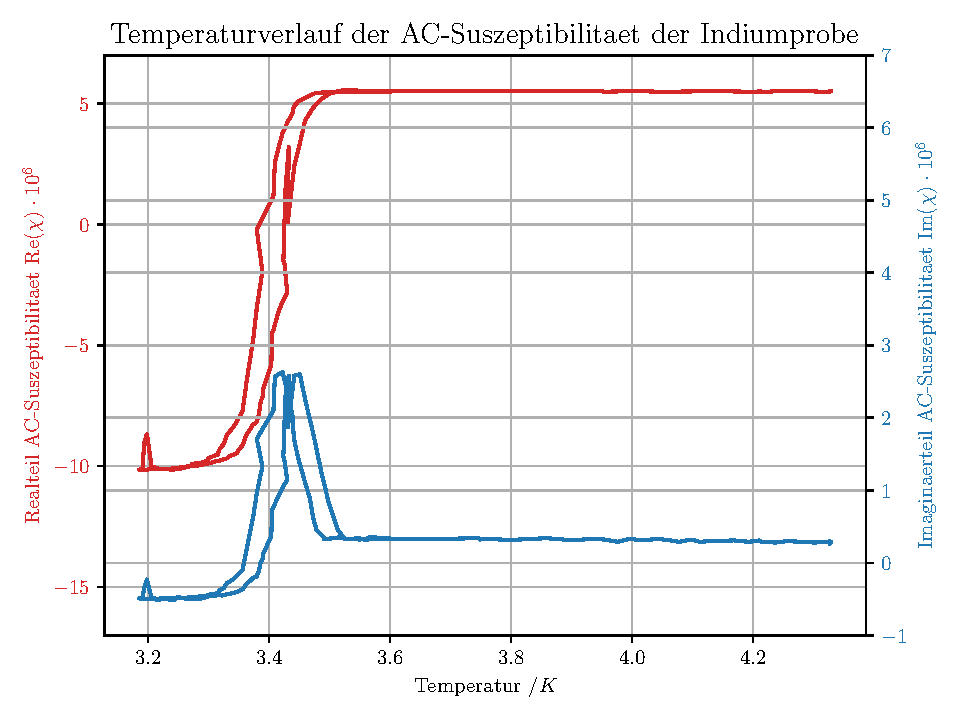
\includegraphics[width=\textwidth]{Temperaturverlauf_der_AC-Suszeptibilitaet_der_Indiumprobe.pdf}

\caption{Temperaturabhängigkeit der komplexen AC-Suszeptibilität der Indiumprobe}
\label{ac-sus}
\end{figure}

Während die Indiumprobe heruntergekühlt wird und sich danach wieder erwärmt, wird mit Hilfe eines magnetischen Wechselfeldes die AC-Suszeptibilität gemessen. In Abbildung \ref{ac-sus} sieht man den Temperaturverlauf der komplexen AC-Suszeptibilität. Auf der linken roten Achse ist der Wert des Realteils der AC-Suszeptibilität dargestellt und auf der rechten blauen Achse der Imaginärteil. Bis zur kritischen Temperatur $T_c$ verlaufen beide Anteile recht konstant. Bei der kritischen Temperatur fällt der Realteil schnell auf einen konstanten negativen Wert ab, während der Imaginärteil einen Peak aufweist und bei niedrigeren Temperaturen auf nahezu 0 absinkt. Der theoretische Wert des Realteils beträgt wie oben beschrieben -1, wir messen jedoch vermutlich nicht den genauen Wert sondern die entsprechende Spannung des Lock-In-Verstärkers, sodass wir uns mit dem konstant negativen Wert zufrieden geben. Der Rückweg zu höheren Temperaturen nimmt einen ähnlichen Verlauf, es ist aber eine kleine Hysterese zu erkennen, die sich durch die thermodynamischen Effekte begründen, d.h. das Thermometer befindet sich nicht im thermodynamischen Gleichgewicht mit der Probe.

Während der Realteil der AC-Suszeptibilität den klassischen Charakter des Supraleiters als idealer Diamagnet zeigt, stellt der Imaginärteil eine Größe für die durch das Magnetfeld in der Probe dissipierte Wirkleistung dar. Die vom Wechselfeld induzierten Ströme sind bei endlichem Widerstand schließlich verlustbehaftet und es wird Leistung abgegeben. Das erklärt auch das Absinken des Imaginärteils in der supraleitenden Phase auf annähernd 0, da das Innere des Supraleiters komplett feldfrei bleibt und so keine Leistung verbraucht werden kann.

\subsection{Temperaturabhängigkeit des Widerstands}
Es wurden vier Messungen bei $I \in {0,100,200,300}$ mA gemacht. Eine Messung startete stets bei großen Temperaturen; durch einen Unterdruck wurde auf $T=2,8$K runtergekühlt und schließlich wieder Helium eingelassen, sodass sich jeweils ein geschlossener Weg in der $R(T)$-Kurve bildet, die aufgenommen wurde. Die die angelegten Ströme sind dabei schon in den Betrag der induzierter Magnetfelder umgerechnet. Da es sich um eine einfache Helmholtzspule mit Radius $R=15$mm, Windungszahl $N=750$ handelt, gilt die Propertionalität

\begin{equation}
B(I) = \frac{4}{5}\sqrt{\frac{4}{5}} \frac{\mu_0 N}{R} I \equiv B_H I
\end{equation}

mit $B_H = 4,495 \cdot 10^{-2}$ T/A (Si-Einheiten, $\mu_0 = 1,2566\cdot 10^{-7}$ N/$A^2$).

\begin{figure}[h]
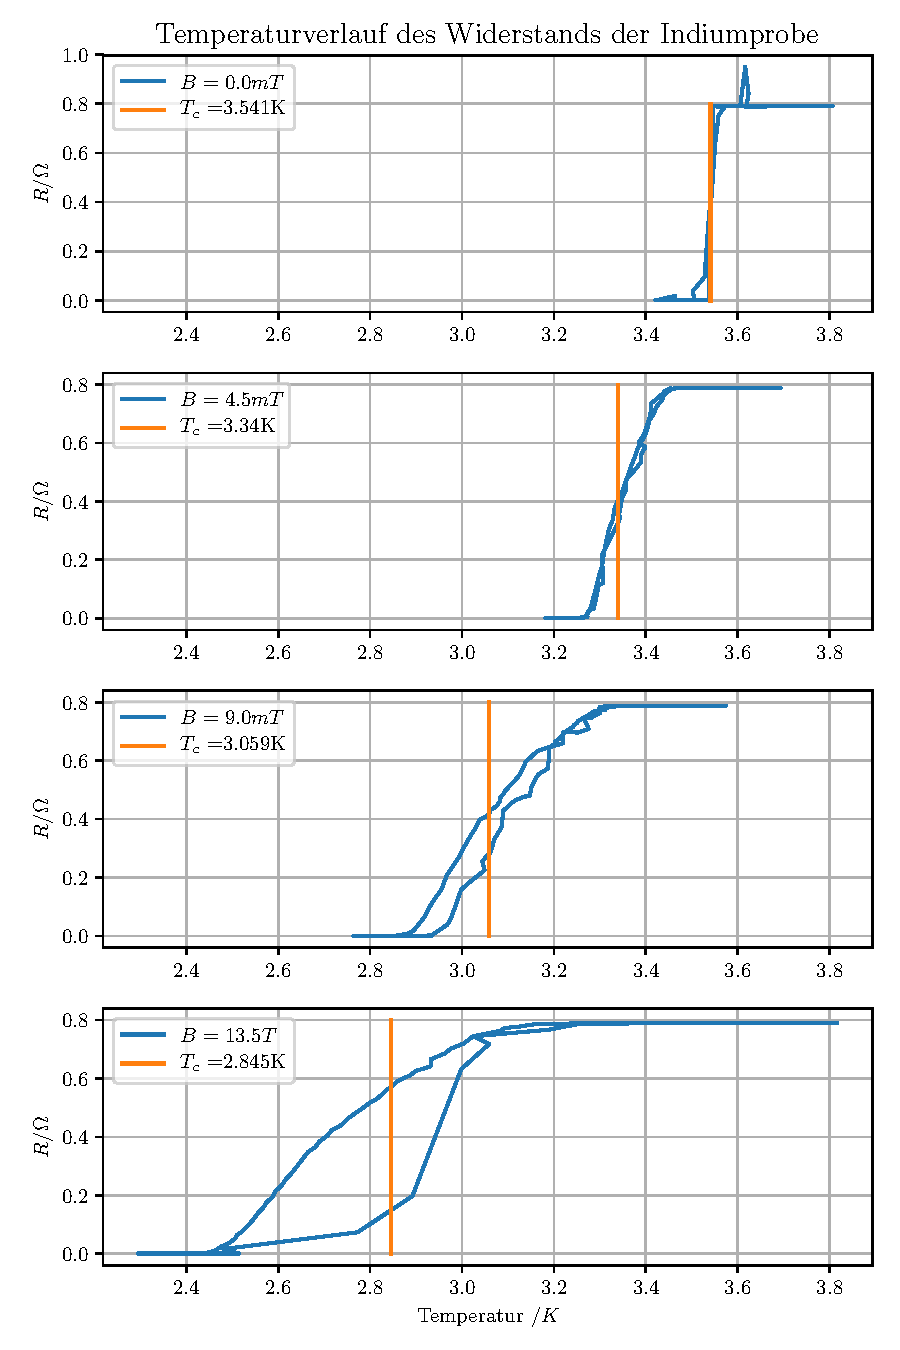
\includegraphics[width=\textwidth]{Temperaturverlauf_des_Widerstands_der_Indiumprobe.pdf}
\end{figure}

Die Graphen zeigen schön den sprunghaften Widerstandsabfall bei der jeweiligen Sprungtemperatur, wobei nur der Übergang bei $B=0$T wirklich als sprunghaft zu bezeichnen ist. In allen anderen Messungen erscheint der Phasenübergang sehr aufgeweitet, wobei wir Verunreinigungen in der Probe als Grund vermuten, die mit steigendem Magnetfeld immer stärker zum Tragen kommen. 


Mit folgender Näherungsgleichung für das Phasendiagramm können die kritischen B-Felder bei $T=0$ für die vier Messgrößen bestimmt werden:

\begin{equation}
B_c(T) = B_c(0) \cdot \left( 1 - \left( T / T_c(0) \right)^2 \right)
\end{equation}

Umgestellt nach $B_c(0) = B_i / (1 - (T / T_{c,0})^2 )$ ergibt das mit der Sprungtemperatur $T_c$ = $T_{c,0}$, die man aus der Tabelle abliest:

\begin{table}[h]
\center\begin{tabular}[h]{|r|r|r|l|l|}
\hline
$i$ & $I_i$ [mA] &  $B_i$ [mT] & $T_{c,i}$ [K] \\
\hline
0 &   0 &       0 & 3,541 \\
1 & 100 &  4,5 & 3,34 \\
2 & 200 &  9 & 3,059 \\
3 & 300 & 13,5 & 2,845 \\
\hline
\end{tabular}
\end{table}

Fittet man die Funktion an diese Werte, erhält man mit geeigneten Ausgangsparametern den Wert $B_c(0) = 37,2 mT$ und damit das interpolierte Phasendiagramm:

\begin{figure}[h]
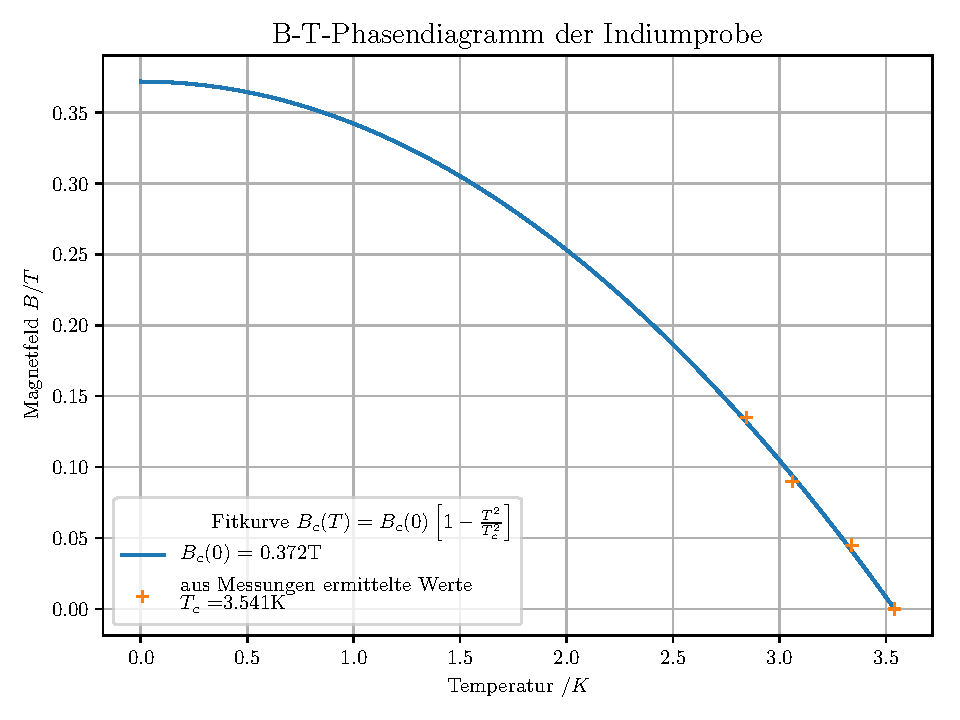
\includegraphics[width=\textwidth]{B-T-Phasendiagramm_der_Indiumprobe.pdf}
\end{figure}

Unser Fit passt wie am Phasendiagramm ersichtlich sehr gut zu den aufgenommenen Daten, und gibt einen guten Wert für das kritische Magnetfeld bei $T=0K$.
Das erweist auch der Vergleich mit dem Literaturwert $ B_{c,\textrm{Lit}}(0) = 29,3\textrm{mT}$, zu dem wir natürlich eine Abweichung feststellen, aber uns durchaus in der richtigen Größenordnung bewegen. 

